\section{Bối cảnh}
\label{sec:context}
Haitay không xuất hiện từ con số không, vì nó kế thừa một công cụ mà mọi cuber đều quen tay. Hiểu cách công cụ ấy hoạt động giúp thấy rõ Haitay giữ lại điều gì và thay đổi điều gì.

\subsection{Stackmat}
Stackmat là bộ hẹn giờ chuẩn tại các giải speedcubing, với dáng thanh ngang dễ nhận ra. Hình~\ref{fig:stackmat} cho thấy cấu tạo của nó: hai pad màu đen nằm ở hai đầu thân máy, mỗi pad in một biểu tượng bàn tay để chỉ chỗ đặt lòng bàn tay, còn mặt hiển thị và các nút điều khiển nằm gọn ở phần giữa.

\begin{figure}[htbp]
    \centering
    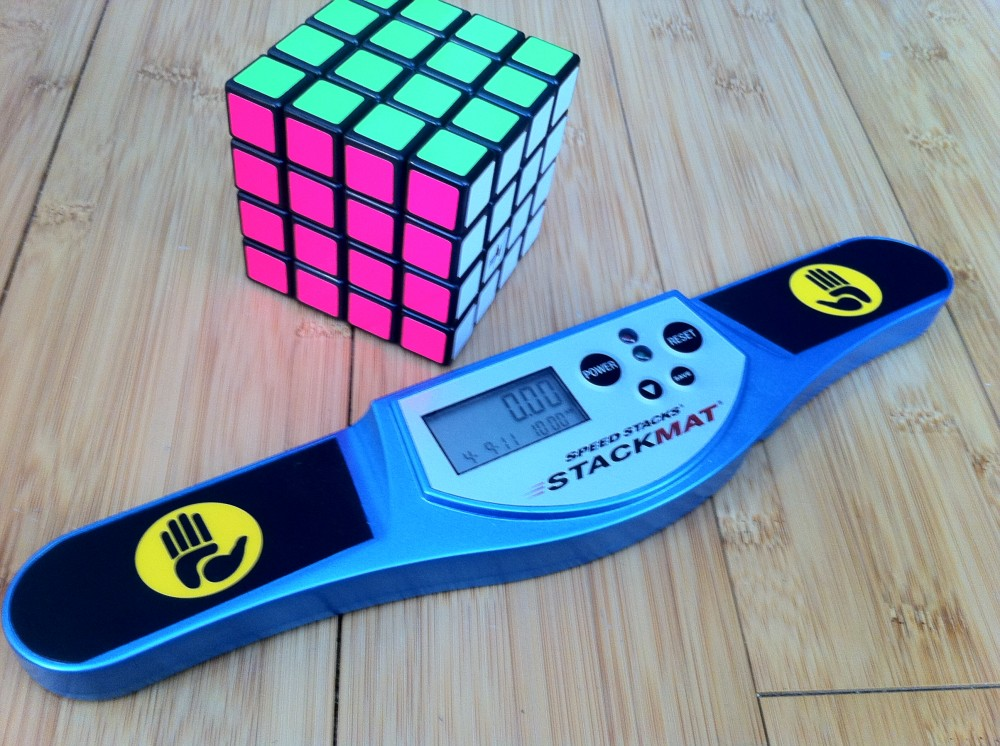
\includegraphics[width=0.78\textwidth]{figures/stackmat.jpg}
    \caption{Stackmat đặt cạnh một khối Rubik 4$\times$4. Hai pad ở hai đầu mang biểu tượng bàn tay. Ảnh của Protocoldoug, giấy phép CC0, nguồn Wikimedia Commons.}
    \label{fig:stackmat}
\end{figure}

Nguyên tắc vận hành của Stackmat xoay quanh việc cố định cả hai tay. Trước lượt solve, người chơi đặt đồng thời hai bàn tay lên hai pad. Khi thiết bị nhận ra cả hai tay đã chạm, nó chuyển sang trạng thái sẵn sàng. Người chơi nhấc một hoặc cả hai tay để bắt đầu giải, và đồng hồ chạy ngay tại thời điểm nhả pad. Giải xong khối, họ đặt cả hai tay trở lại pad để dừng đồng hồ.\footnote{Theo quy tắc StackMat Pro của WSSA: \url{https://www.thewssa.com/docs/rules_rules.pdf}.}

Cách cố định này giải quyết hai vấn đề cùng lúc. Trước hết, cả hai tay đều rời khối Rubik trước khi đồng hồ chạy, nên mọi người bắt đầu từ cùng một điểm xuất phát. Kế đó, người chơi phải buông khối bằng cả hai tay mới dừng được đồng hồ, nên thời gian dừng phản ánh đúng lúc khối được giải xong. Một nút bấm duy nhất khó đạt được hai điều này, và đó là lý do cơ chế hai pad được giữ lại ở Haitay.

% Chừa chỗ: luật thi đấu WCA liên quan đến bấm giờ, bổ sung sau.
